% ~~~~~~~~~~~~~~~~~~~~~~~~~~~~~~~~~~~~
% EXAMPLE SIMULATION EXPERIMENT
% ~~~~~~~~~~~~~~~~~~~~~~~~~~~~~~~~~~~~
\section{Example simulation experiment (repressilator.omex)}
\label{example:repressilator}
This example lists the SED-ML corresponding to the motivational example in the introduction (Section~\ref{motivation:example}), which provides a description of the executed simulation experiment and the used repressilator model. 

\myXmlImport{SED-ML document for example simulation experiment.}
{lst:repressilator}
{examples/repressilator/repressilator.xml}

% ~~~~~~~~~~~~~~~~~~~~~~~~~~~~~~~~~~~~
% IKAPPAB
% ~~~~~~~~~~~~~~~~~~~~~~~~~~~~~~~~~~~~
%\section{IkappaB-NF-kappaB Signaling (SBML)}
%The following example provides a SED-ML description for the simulation of the IkappaB-NF-kappaB signaling module based on the publication by Hoffmann, Levchenko, Scott and  Baltimore ``The IkappaB-NF-kappaB signaling module: temporal control and selective gene activation.'' (PubMed ID: 12424381)
%
%This model is referenced by its SED-ML ID \code{model1} and refers to the model with the MIRIAM URN \url{urn:miriam:biomodels.db:BIOMD0000000140}. 
%Software applications interpreting this example know how to dereference this URN and access the model in \biom \citep{N+06}.
%
%The simulation description specifies one simulation \code{simulation1}, which is a uniform timecourse simulation that simulates the model for 41 hours. \code{task1} then applies this simulation to the model. 
%
%As output this simulation description collects four parameters: \code{Total\_NFkBn}, \code{Total\_IkBbeta}, \code{Total\_IkBeps} and \code{Total\_IkBalpha}. These variables are to be plotted against the simulation time and displayed in four separate plots, as shown in Figure \ref{fig:ikappab}. 
%
%\sedfig[width=0.8\textwidth]{examples/ikappab/ikappab}{The simulation result gained from the simulation description given in \lst{ikappab}}{fig:ikappab}
%
%The SED-ML description of the simulation experiment is given in \lst{ikappab}.
%
%\myXmlImport{IkappaB-NF-kappaB signaling Model Simulation Description in SED-ML}{lst:ikappab}{examples/ikappab/ikappab.xml}

% ~~~~~~~~~~~~~~~~~~~~~~~~~~~~~~~~~~~~
% DATA EXAMPLES
% ~~~~~~~~~~~~~~~~~~~~~~~~~~~~~~~~~~~~
\section{Simulation experiments with dataDescriptions}
The \hyperref[class:dataDescription]{DataDescription} make it possible to work with external data in simulation experiments. In this section simulation experiments using the \hyperref[class:dataDescription]{dataDescription} are presented.

\subsection{Reading data as NUML or CSV (\code{reading-data-numl.omex} and \code{reading-data-csv.omex})}
This examples demonstrate the use of the \hyperref[class:dataDescription]{DataDescription} and \hyperref[class:dataSource]{DataSource} to load external data in SED-ML. 

%\sedfigX[scale=0.6]{examples/reading-data-csv/results/reading-data-csv}{Loaded and plotted data from the simulation description given in \lst{reading-data-csv}}{fig:reading-data-csv}
\begin{figure}[ht]
    \centering
    \begin{minipage}{0.47\textwidth}
        \centering
        
\includegraphics[width=1.0\textwidth]{examples/placeholder}
        \caption{Loaded and plotted data from the simulation description given in \lst{reading-data-csv} with SED-ML webtools.}
    \end{minipage}\hfill
    \begin{minipage}{0.47\textwidth}
        \centering
        
\includegraphics[width=1.0\textwidth]{examples/placeholder}
        \caption{Loaded and plotted data from the simulation description given in \lst{reading-data-csv} with tellurium.}
    \end{minipage}
    \label{fig:reading-data-csv}
\end{figure}

\myXmlImport{SED-ML document using \SedDataSource and \SedDataDescription}
{lst:reading-data-csv}
{examples/reading-data-csv/reading-data-csv.xml}

\subsection{Plotting data with simulations (\code{plotting-data.omex})}
This example demonstrates the use of the \hyperref[class:dataDescription]{DataDescription} and \hyperref[class:dataSource]{DataSource} to load external data in SED-ML. In the example a \hyperref[class:model]{model} is simulated (using a \hyperref[class:uniformTimeCourse]{uniformTimeCourse} simulation), the simulation result is plotted in one plot. A second plot obtains a stored result (using the \hyperref[class:dataDescription]{dataDescription} and \hyperref[class:dataSource]{DataSource}), extracts the \token{S1} and \token{time} column from it and renders it.

%\sedfigX[scale=0.6]{examples/plotting-data/results/plotting-data}{The simulation result from the simulation description given in \lst{plotting-data}}{fig:plotting-data}

\begin{figure}[ht]
    \centering
    \begin{minipage}{0.47\textwidth}
        \centering
        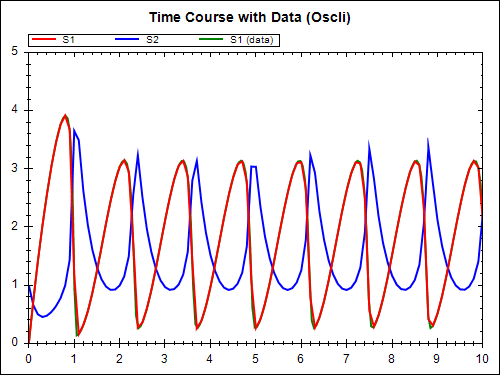
\includegraphics[width=1.0\textwidth]{examples/plotting-data/results/sedml_webtools/timecourse_with_data}
        \caption{The simulation result from the simulation description given in \lst{plotting-data} with SED-ML webtools.}
    \end{minipage}\hfill
    \begin{minipage}{0.47\textwidth}
        \centering
        
\includegraphics[width=1.0\textwidth]{examples/placeholder}
        \caption{The simulation result from the simulation description given in \lst{plotting-data} with tellurium.}
    \end{minipage}
    \label{fig:plotting-data}
\end{figure}

\myXmlImport{SED-ML document using \SedDataSource and \SedDataDescription}
{lst:plotting-data}
{examples/plotting-data/plotting-data.xml}

% ~~~~~~~~~~~~~~~~~~~~~~~~~~~~~~~~~~~~
% REPEATED TASKS
% ~~~~~~~~~~~~~~~~~~~~~~~~~~~~~~~~~~~~
\section{Simulation experiments with repeatedTasks}
The \hyperref[class:repeatedTask]{repeatedTask} makes it possible to encode a large number of different simulation experiments. In this section several such simulation experiments using the \hyperref[class:repeatedTask]{repeatedTask} are presented.

% ~~~ TIME COURSE PARAMETER SCAN ~~~
\subsection{Time course parameter scan (\code{repeated-scan-oscli.omex})}
In this example a \hyperref[class:repeatedTask]{repeatedTask} is used to run repeated \hyperref[class:uniformTimeCourse]{uniformTimeCourse} simulations with a deterministic simulation algorithm. Within the \hyperref[class:repeatedTask]{repeatedTask} after each run the parameter value is changed, resulting in a time course parameter scan.

NOTE: This example produces three dimensional results (time, species concentration, multiple repeats).  SED-ML \currentLV does not include a way to post-process these values, so it is left to the implementation on how to display them. One example would be to flatten the values by overlaying them onto the desired plot. 

%\sedfigX[scale=0.6]{examples/repeated-scan-oscli/results/repeated-scan-oscli}{The simulation result gained from the simulation description given in \lst{repeated-scan-oscli}}{fig:repeated-scan-oscli}

\begin{figure}[ht]
    \centering
    \begin{minipage}{0.47\textwidth}
        \centering
        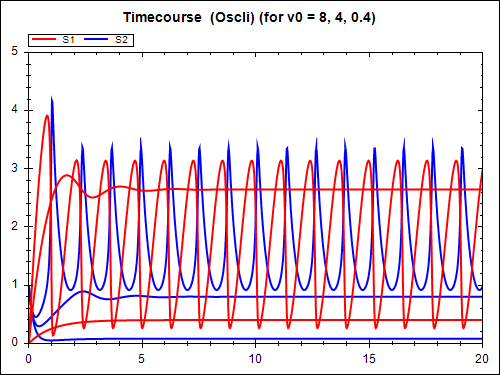
\includegraphics[width=1.0\textwidth]{examples/repeated-scan-oscli/results/sedml_webtools/plot1}
        \caption{The simulation result gained from the simulation description given in \lst{repeated-scan-oscli} with SED-ML webtools.}
    \end{minipage}\hfill
    \begin{minipage}{0.47\textwidth}
        \centering
        
\includegraphics[width=1.0\textwidth]{examples/placeholder}
        \caption{The simulation result gained from the simulation description given in \lst{repeated-scan-oscli} with tellurium.}
    \end{minipage}
    \label{fig:repeated-scan-oscli}
\end{figure}

\myXmlImport{SED-ML document implementing the one dimensional time course parameter scan}
{lst:repeated-scan-oscli}
{examples/repeated-scan-oscli/repeated-scan-oscli.xml}

% ~~~ STEADY STATE PARAMETER SCAN ~~~
\subsection{Steady state parameter scan (\code{repeated-steady-scan-oscli.omex})}
In this example a \hyperref[class:repeatedTask]{repeatedTask} is used in combination with a \hyperref[class:steadyState]{steadyState} simulation task (performing a steady state computation). On each repeat a parameter is varied resulting in a steady state parameter scan.

%\sedfigX[scale=0.6]{examples/repeated-steady-scan-oscli/results/repeated-steady-scan-oscli}{The simulation result from the simulation description given in \lst{repeated-steady-scan-oscli}}{fig:figrepeated1}

\begin{figure}[ht]
    \centering
    \begin{minipage}{0.47\textwidth}
        \centering
        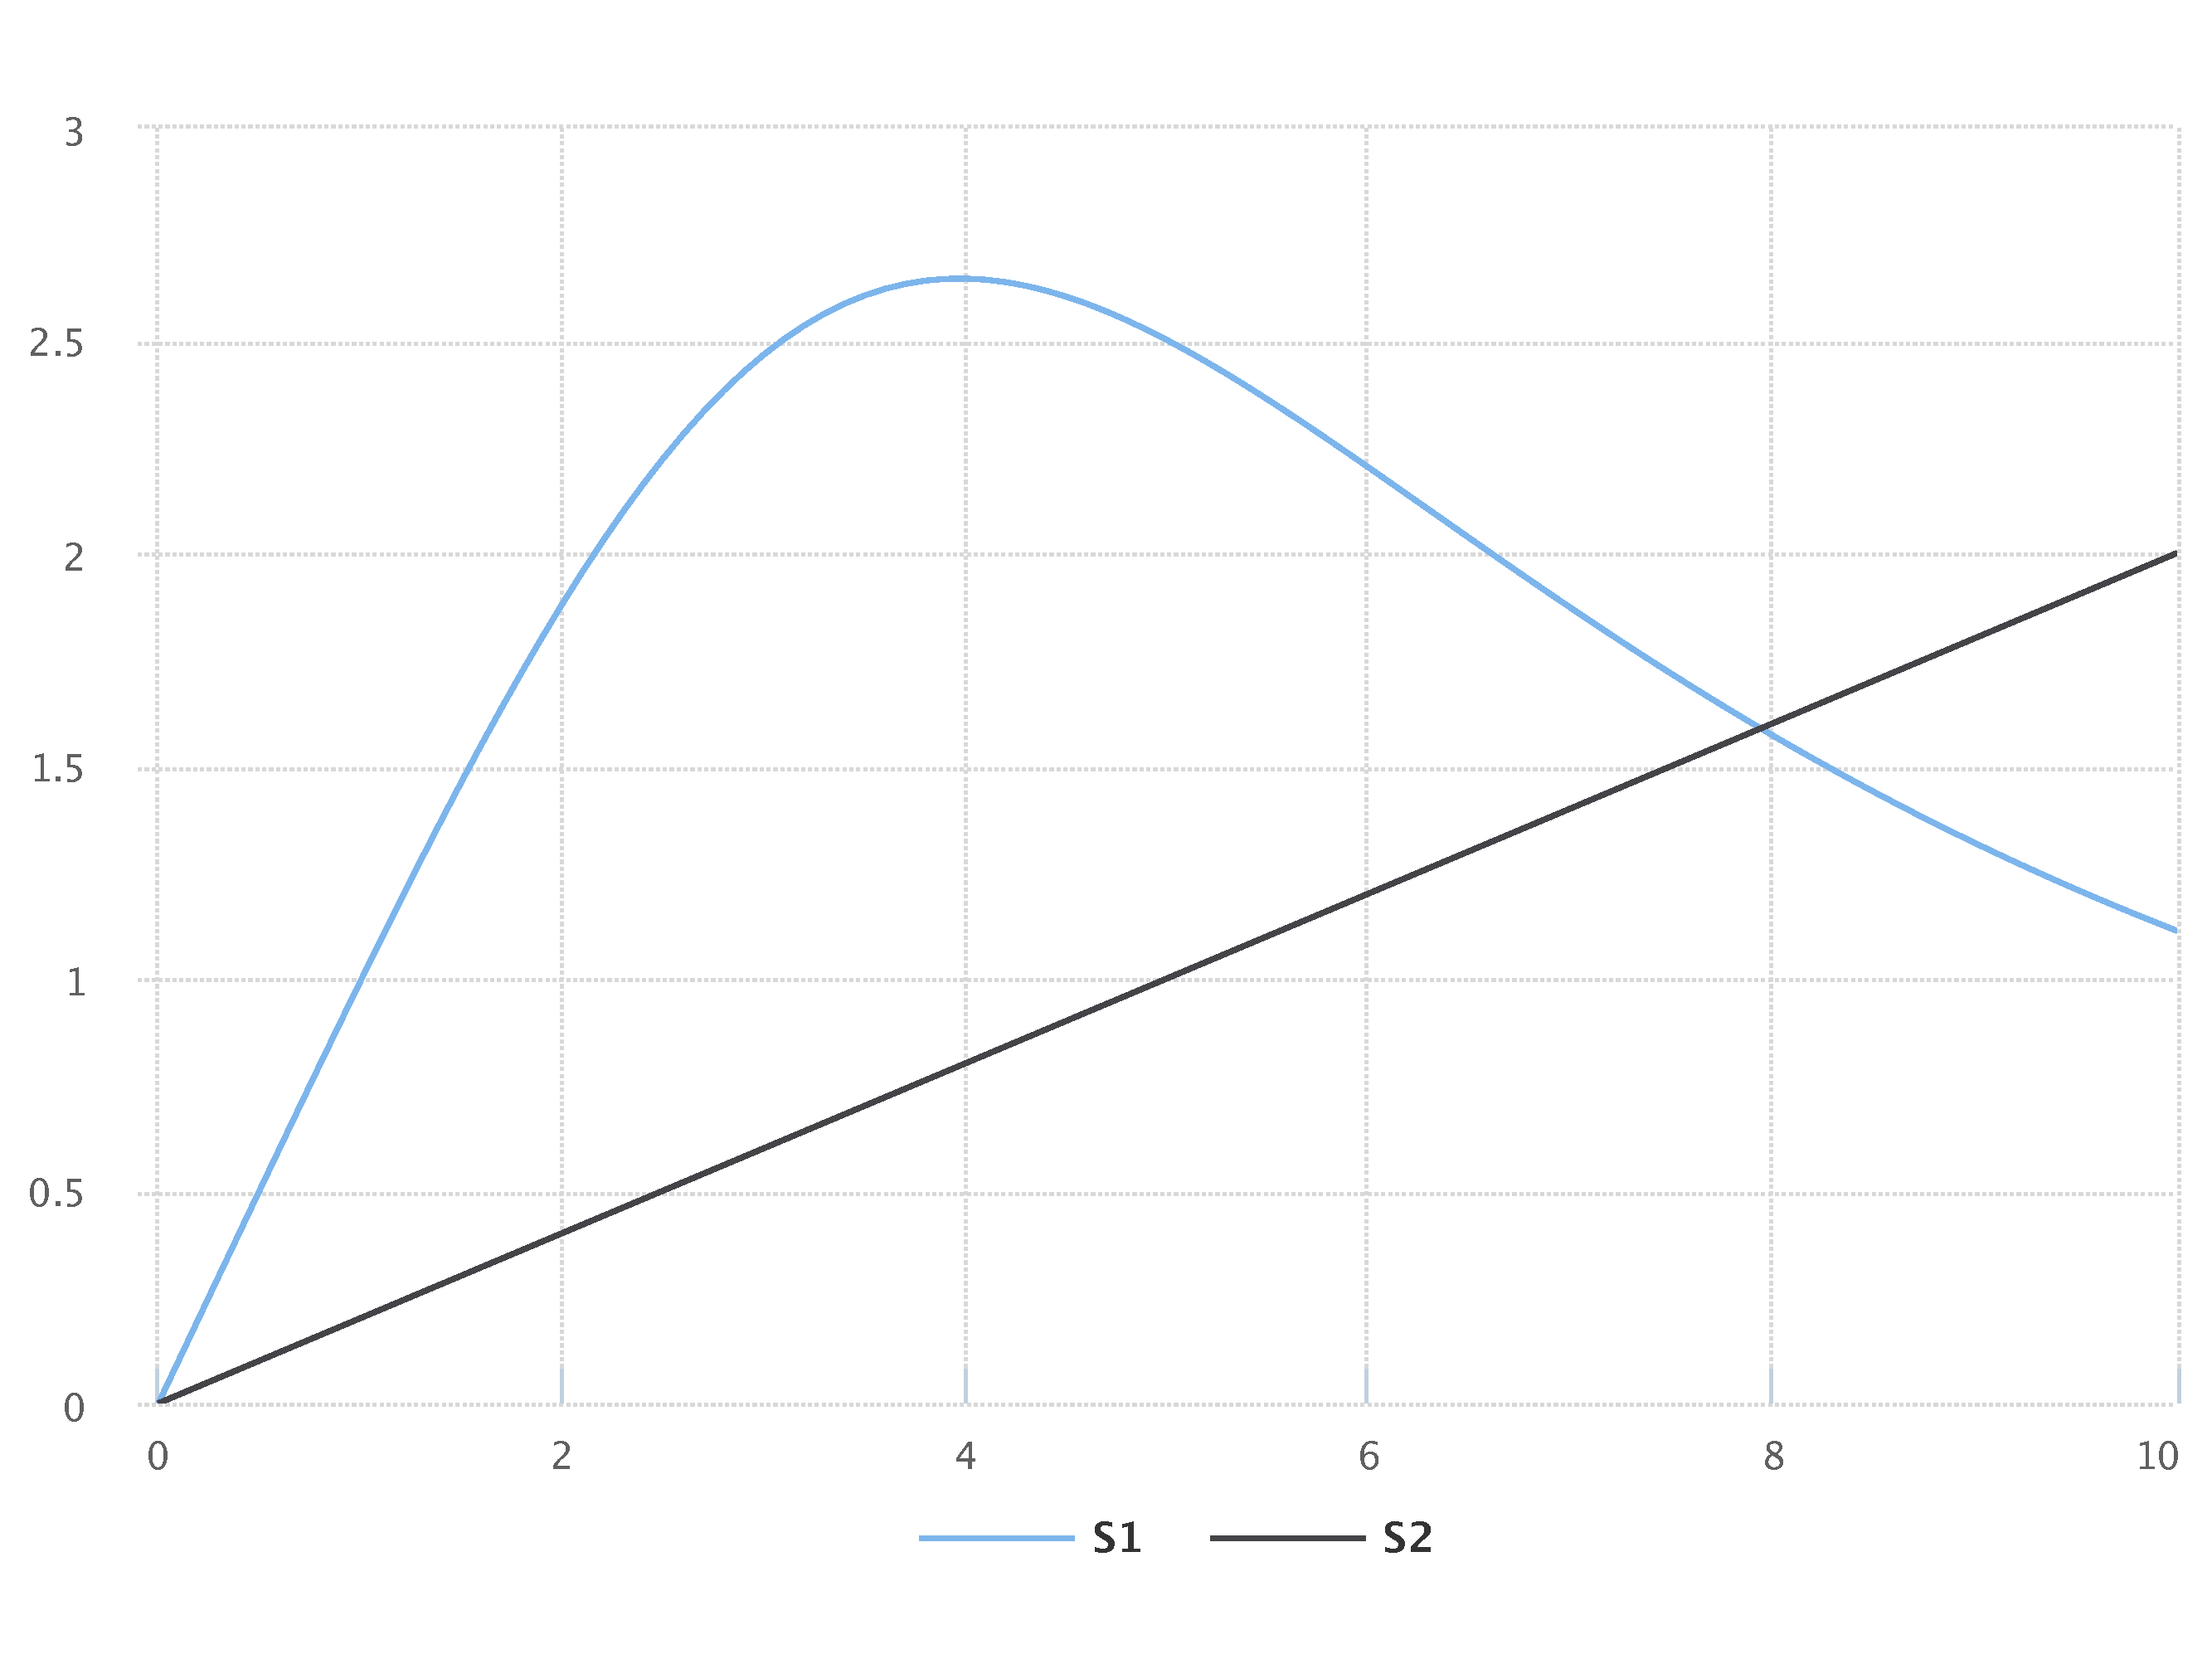
\includegraphics[width=1.0\textwidth]{examples/repeated-steady-scan-oscli/results/sedml_webtools/plot1}
        \caption{The simulation result from the simulation description given in \lst{repeated-steady-scan-oscli} with SED-ML webtools.}
    \end{minipage}\hfill
    \begin{minipage}{0.47\textwidth}
        \centering
        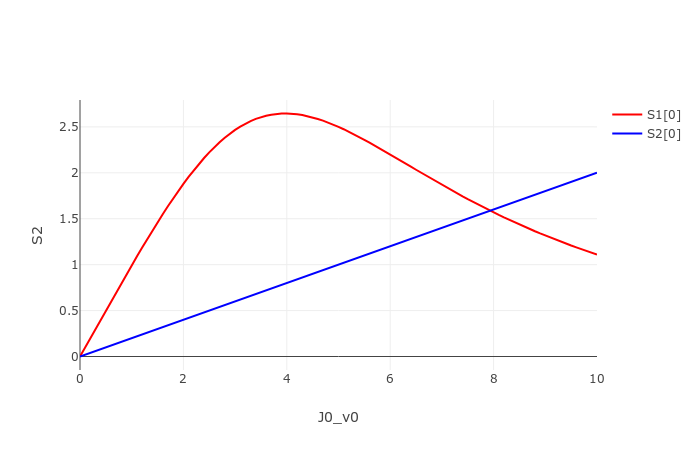
\includegraphics[width=1.0\textwidth]{examples/repeated-steady-scan-oscli/results/tellurium/plot1}
        \caption{The simulation result from the simulation description given in \lst{repeated-steady-scan-oscli} with tellurium.}
    \end{minipage}
    \label{fig:repeated-steady-scan-oscli}
\end{figure}

\myXmlImport{SED-ML document implementing the one dimensional steady state parameter scan}
{lst:repeated-steady-scan-oscli}
{examples/repeated-steady-scan-oscli/repeated-steady-scan-oscli.xml}


% ~~~ STOCHASTIC SIMULATION ~~~
\subsection{Stochastic simulation (\code{repeated-stochastic-runs.omex})}
In this example a \hyperref[class:repeatedTask]{repeatedTask} is used to run a stochastic simulation multiple times.
Running just one stochastic trace does not provide a complete picture of the behavior of a system. A large number of traces are needed. This example demonstrates the basic use case of running ten traces of a simulation by using a \hyperref[class:repeatedTask]{repeatedTask} which runs ten uniform time course simulations (each performing a stochastic simulation run).

NOTE: This example produces three dimensional results (time, species concentration, multiple repeats). While SED-ML \currentLV does not include a way to post-processing these values. So it is left to the implementation on how to display them. One example would be to flatten the values by overlaying them onto the desired plot. 

%\sedfigX[scale=0.6]{examples/repeated-stochastic-runs/results/repeated-stochastic-runs}{The simulation result from the simulation description given in \lst{repeated-stochastic-runs}}{fig:repeated-stochastic-runs}

\begin{figure}[ht]
    \centering
    \begin{minipage}{0.47\textwidth}
        \centering
        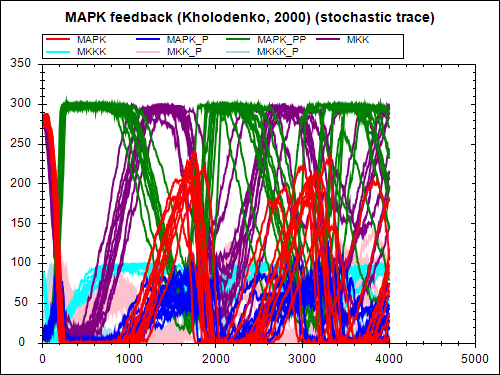
\includegraphics[width=1.0\textwidth]{examples/repeated-stochastic-runs/results/sedml_webtools/plot1}
        \caption{The simulation result from the simulation description given in \lst{repeated-stochastic-runs} with SED-ML webtools.}
    \end{minipage}\hfill
    \begin{minipage}{0.47\textwidth}
        \centering
        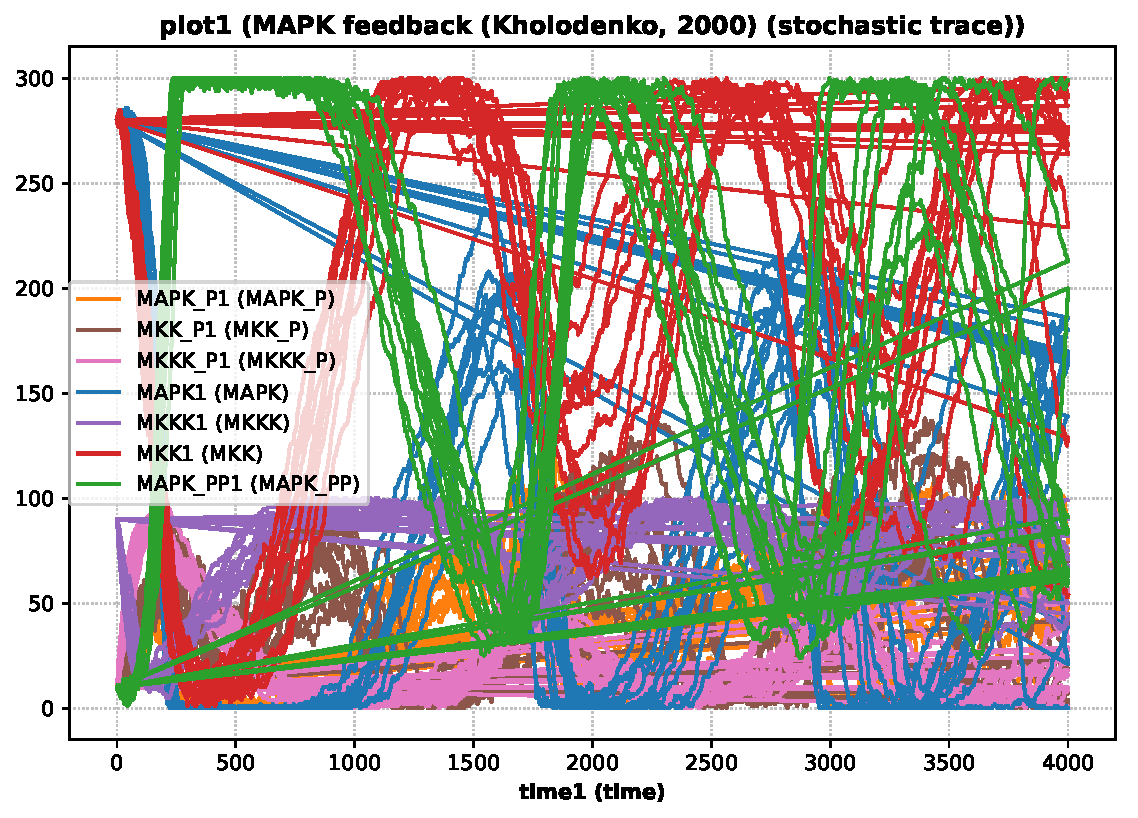
\includegraphics[width=1.0\textwidth]{examples/repeated-stochastic-runs/results/tellurium/plot1}
        \caption{The simulation result from the simulation description given in \lst{repeated-stochastic-runs} with tellurium.}
    \end{minipage}
    \label{fig:repeated-stochastic-runs}
\end{figure}

\myXmlImport{SED-ML document implementing repeated stochastic runs}
{lst:repeated-stochastic-runs}
{examples/repeated-stochastic-runs/repeated-stochastic-runs.xml}


% ~~~ SIMULATION PERTURBATION ~~~
\subsection{Simulation perturbation (\code{oscli-netsted-pulse.omex})}
Often it is interesting to see how the dynamic behavior of a model changes when some perturbations are applied to the model. In this example a \hyperref[class:repeatedTask]{repeatedTask} is used iterating a \hyperref[class:oneStep]{oneStep} task (that advances an ODE integration to the next output step). During the steps a single parameter is modified effectively causing the oscillations of a model to stop. Once the value is reset the oscillations recover. 

Note: In the example a \hyperref[class:functionalRange]{functionalRange} is used, although the same result could also be achieved using the \hyperref[class:setValue]{setValue} element directly.

%\sedfigX[scale=0.6]{examples/oscli-nested-pulse/results/oscli-nested-pulse}{The simulation result from the simulation description given in \lst{oscli-nested-pulse}}{fig:oscli-nested-pulse}

\begin{figure}[ht]
    \centering
    \begin{minipage}{0.47\textwidth}
        \centering
        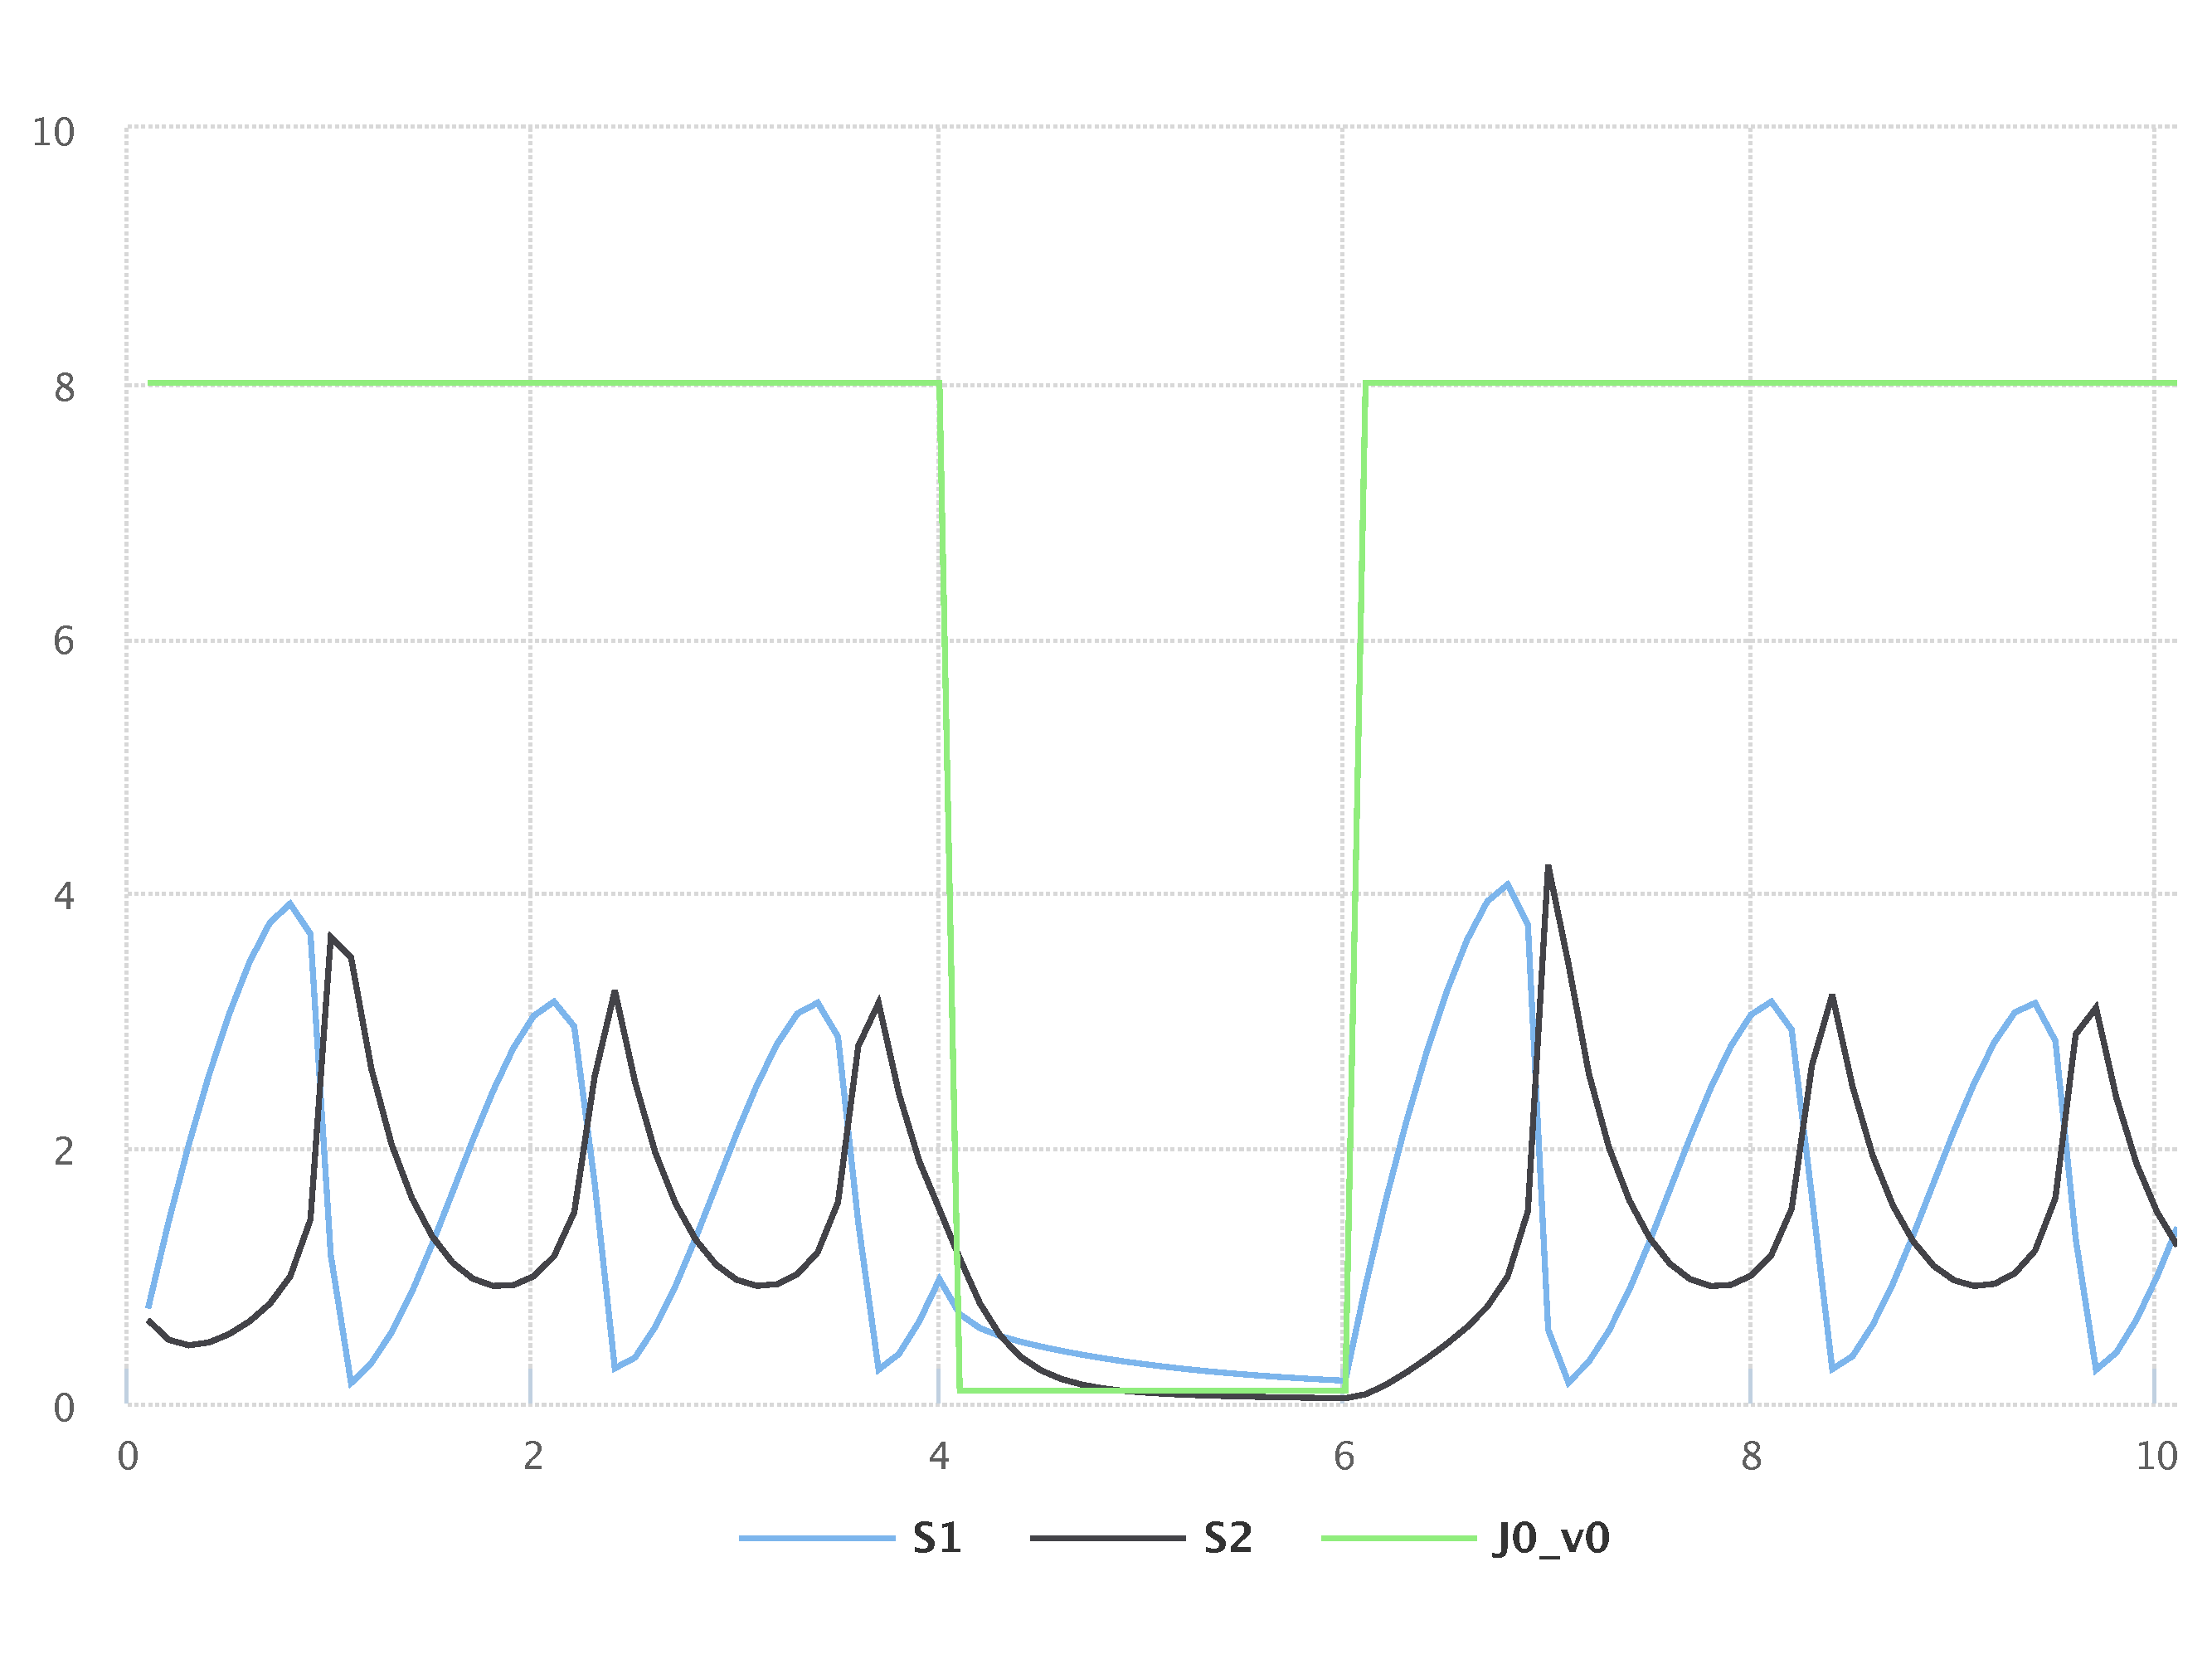
\includegraphics[width=1.0\textwidth]{examples/oscli-nested-pulse/results/sedml_webtools/plot1}
        \caption{The simulation result from the simulation description given in \lst{oscli-nested-pulse} with SED-ML webtools.}
    \end{minipage}\hfill
    \begin{minipage}{0.47\textwidth}
        \centering
        
\includegraphics[width=1.0\textwidth]{examples/placeholder}
        \caption{The simulation result from the simulation description given in \lst{oscli-nested-pulse} with tellurium.}
    \end{minipage}
    \label{fig:oscli-nested-pulse}
\end{figure}

\myXmlImport{SED-ML document implementing the perturbation experiment}
{lst:oscli-nested-pulse}
{examples/oscli-nested-pulse/oscli-nested-pulse.xml}


% ~~~ 2D STEADY STATE PARAMETER SCAN ~~~
\subsection{2D steady state parameter scan (\code{parameter-scan-2d.omex})}
In this example a \hyperref[class:repeatedTask]{repeatedTask} which runs over another \hyperref[class:repeatedTask]{repeatedTask} which performs a steady state computation. Each repeated simulation task modifies a different parameter.

NOTE: This example produces three dimensional results (time, species concentration, multiple repeats). While SED-ML \currentLV does not include a way to post-processing these values. So it is left to the implementation on how to display them. One example would be to flatten the values by overlaying them onto the desired plot. 

%\sedfigX[width=0.7\textwidth]{examples/parameter-scan-2d/results/parameter-scan-2d}{The simulation result gained from the simulation description given in \lst{parameter-scan-2d}}{fig:parameter-scan-2d}

\begin{figure}[ht]
    \centering
    \begin{minipage}{0.47\textwidth}
        \centering
        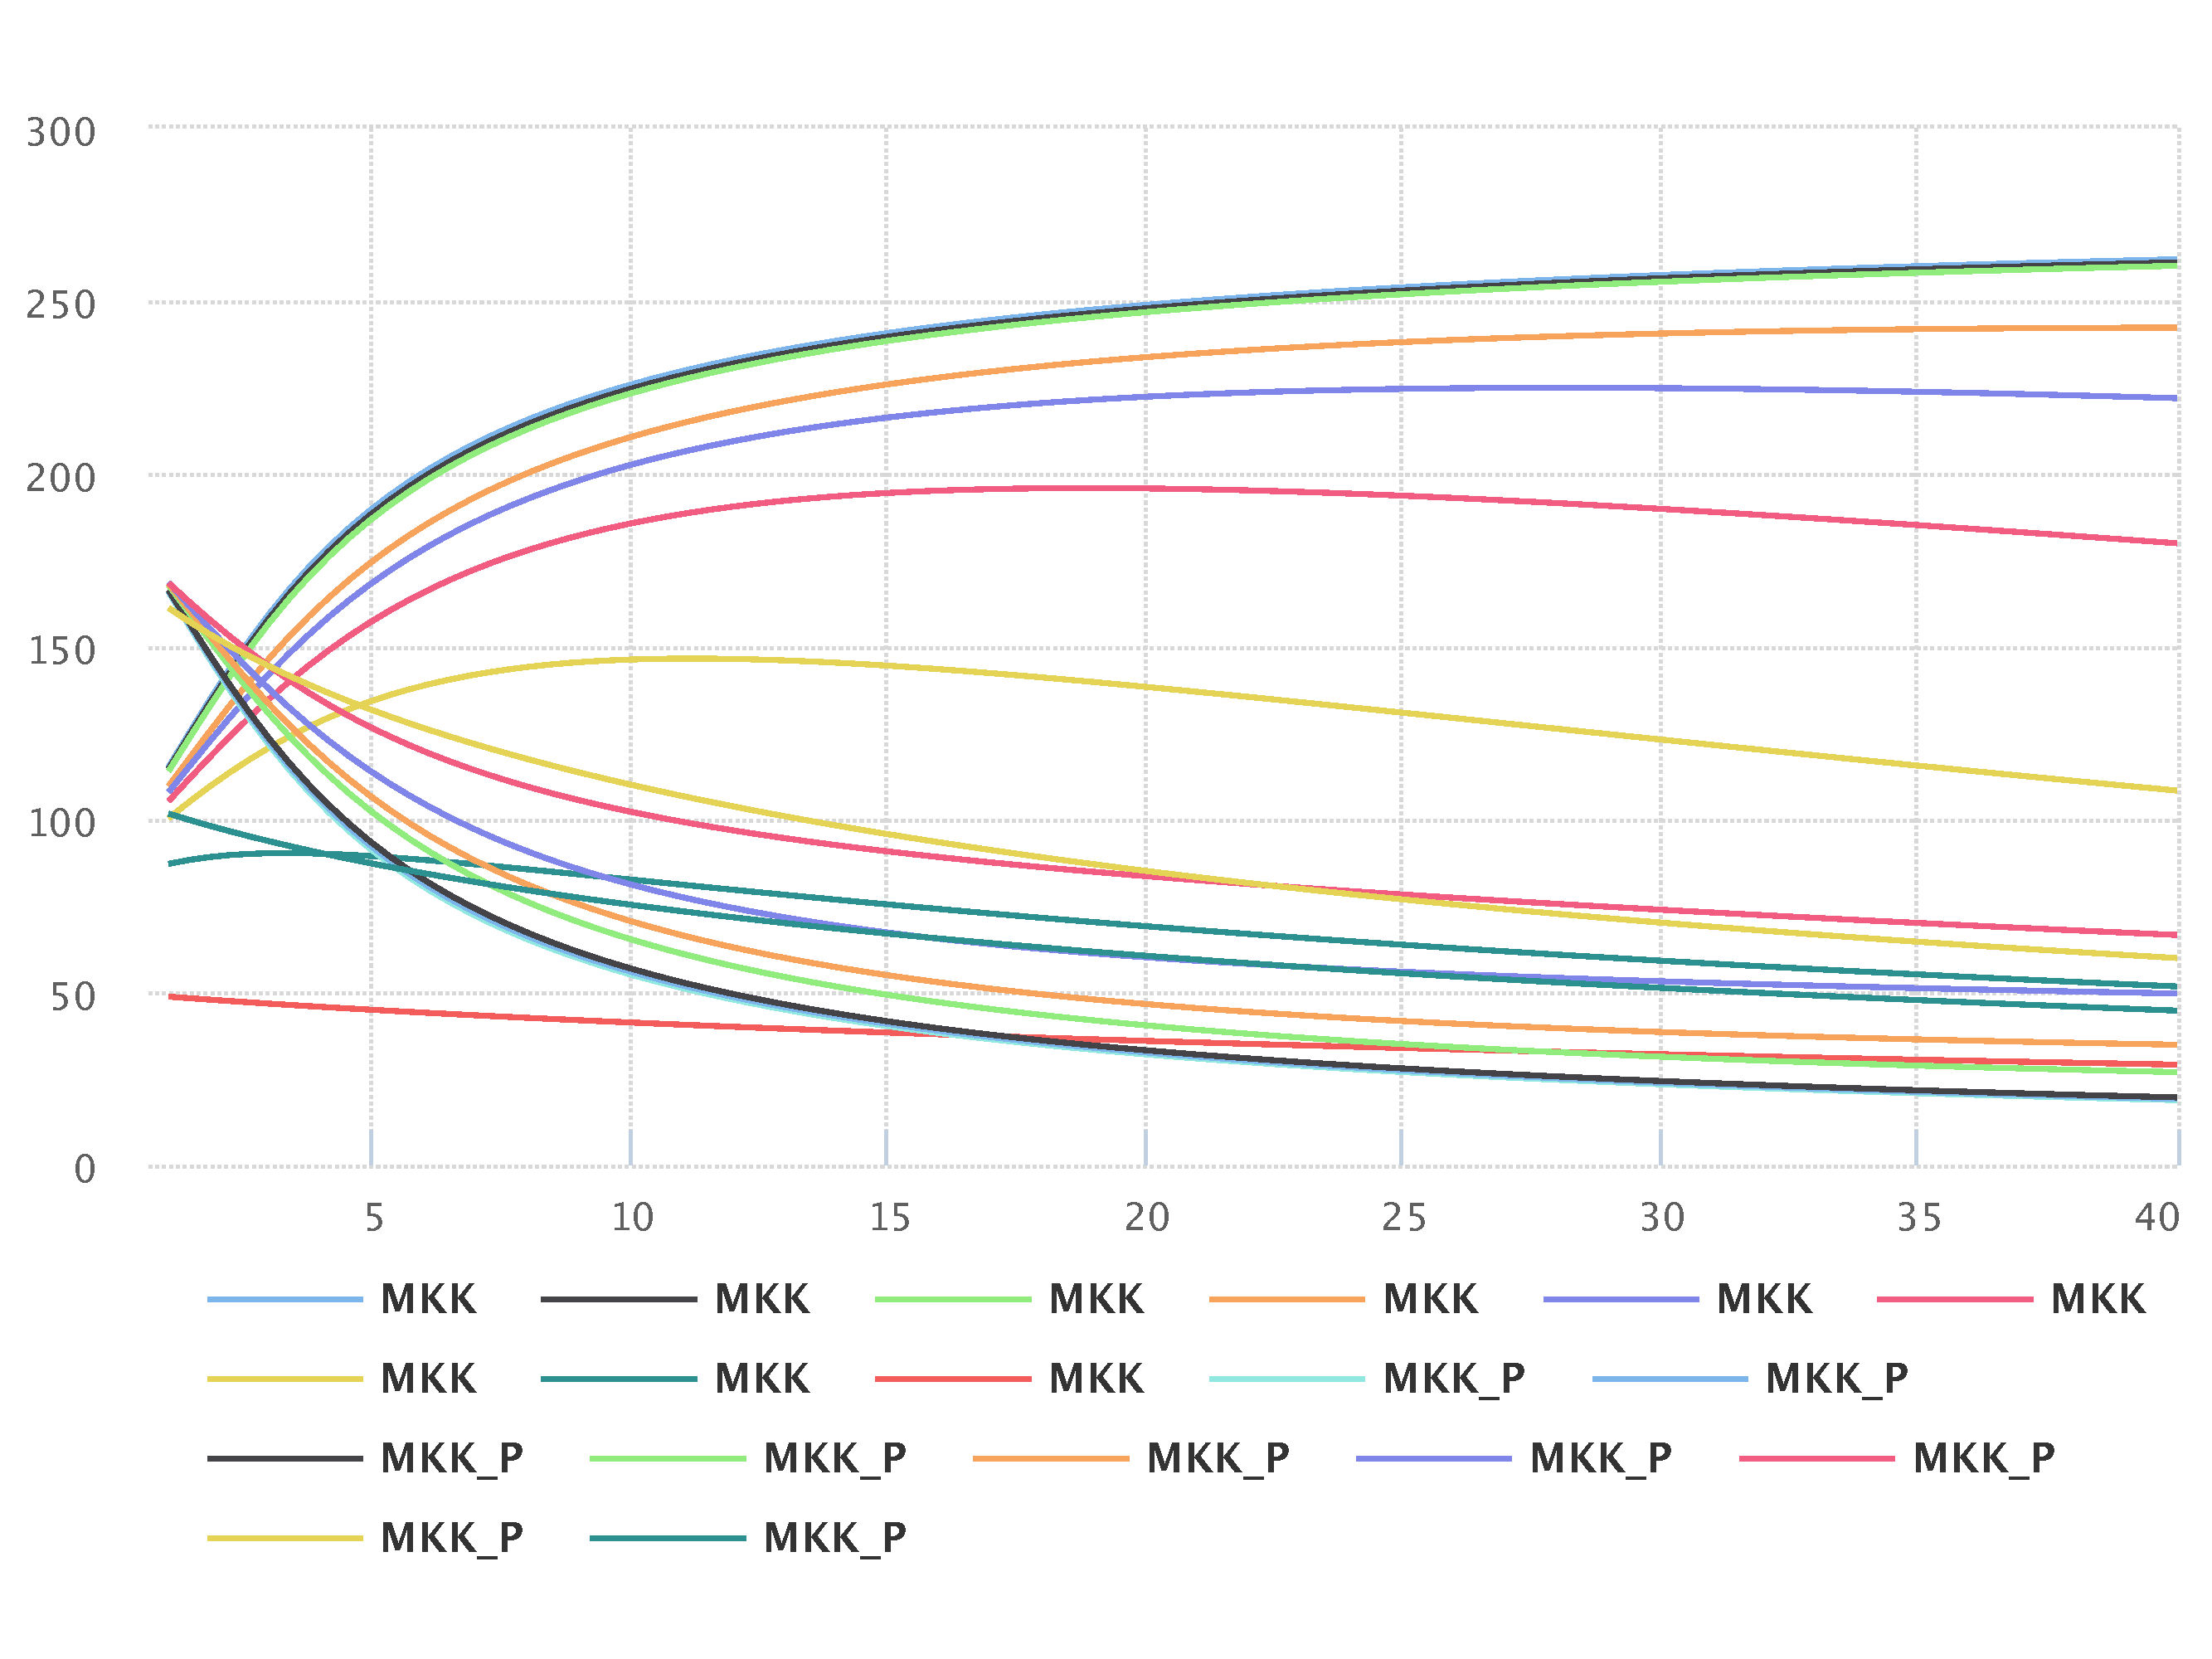
\includegraphics[width=1.0\textwidth]{examples/parameter-scan-2d/results/sedml_webtools/plot1}
        \caption{The simulation result gained from the simulation description given in \lst{parameter-scan-2d} with SED-ML webtools.}
    \end{minipage}\hfill
    \begin{minipage}{0.47\textwidth}
        \centering
        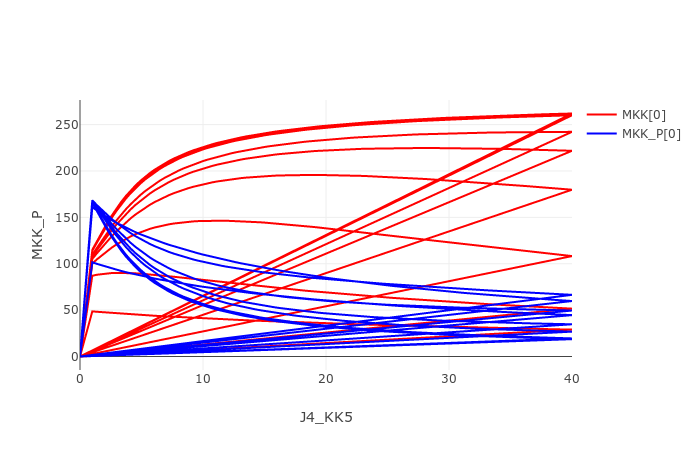
\includegraphics[width=1.0\textwidth]{examples/parameter-scan-2d/results/tellurium/plot1}
        \caption{The simulation result gained from the simulation description given in \lst{parameter-scan-2d} with tellurium.}
    \end{minipage}
    \label{fig:parameter-scan-2d}
\end{figure}

\myXmlImport{SED-ML document implementing the one dimensional steady state parameter scan}
{lst:parameter-scan-2d}
{examples/parameter-scan-2d/parameter-scan-2d.xml}


% ~~~~~~~~~~~~~~~~~~~~~~~~~~~~~~~~~~~~
% DIFFERENT MODEL LANGUAGES
% ~~~~~~~~~~~~~~~~~~~~~~~~~~~~~~~~~~~~
\section{Simulation experiments with different model languages}
SED-ML allows to specify models in various languages, e.g.\ SBML and CellML (see Section~\ref{sec:languageURI} for more information). This section demonstrates the same simulation experiment with the model either in SBML (Appendix~\ref{example:leloup_sbml}) or in CellML (Appendix~\ref{example:leloup_cellml}).

% ~~~ LE LOUP (SBML) ~~~
\subsection{Le Loup Model SBML (\code{leloup-sbml.omex})}
\label{example:leloup_sbml}
The following example provides a SED-ML description for the simulation of the model based on the publication\cite{LeLoup1999}.

The model is referenced by its SED-ML \hyperref[sec:id]{\element{id}} \code{model1} and refers to the model with the MIRIAM URN \url{urn:miriam:biomodels.db:BIOMD0000000021}. A second model is defined in the example, using \code{model1} as a source and applying additional changes to it, in this case updating two model parameters.

One simulation setup is defined in the \code{listOfSimulations}. It is a \code{uniformTimeCourse} over 380 time units, providing 1000 output points. The algorithm used is the CVODE solver, as denoted by the KiSAO ID \code{KiSAO:0000019}.

A number of \hyperref[class:dataGenerator]{dataGenerators} are defined, which are the prerequisite for defining the simulation \hyperref[class:output]{output}. The first \hyperref[class:dataGenerator]{dataGenerator} with \hyperref[sec:id]{\element{id}} \code{time} collects the simulation time. \code{tim1} maps on the \code{Mt} entity in the model that is used in \code{task1} which in the model \code{model1}. The dataGenerator named \code{\texttt{per\_tim1}} maps on the \code{Cn} entity in \code{model1}. Finally  the fourth and fifth dataGenerators map on the \code{Mt} and \code{\texttt{per\_tim}} entity respectively in the updated model with ID \code{model2}.

The \hyperref[class:output]{output} defined in the experiment consists of three \hyperref[class:plot2D]{2D plots}. The first plot has two \hyperref[class:curve]{curves} and provides the time course of the simulation using the tim mRNA concentrations from both tasks. The second plot shows the \code{\texttt{per\_tim}} concentration against the \code{tim} concentration for the oscillating model. The third plot shows the same plot for the chaotic model. The resulting three plots are depicted in Figure \ref{fig:leloup-sbml}. 

%\sedfigX[scale=0.8]{examples/leloup-sbml/results/leloup-sbml}{The simulation result gained from the simulation description given in \lst{leloup-sbml}}{fig:leloup-sbml}

\begin{figure}[ht]
    \centering
    \begin{minipage}{0.47\textwidth}
        \centering
        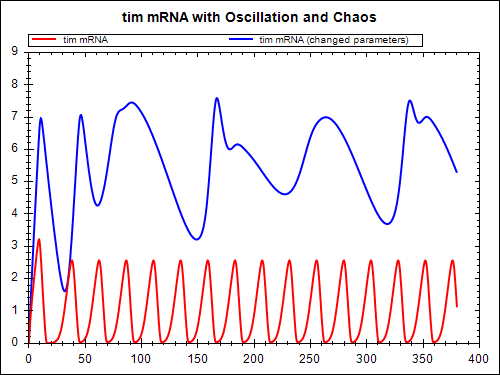
\includegraphics[width=1.0\textwidth]{examples/leloup-sbml/results/sedml_webtools/plot1}
         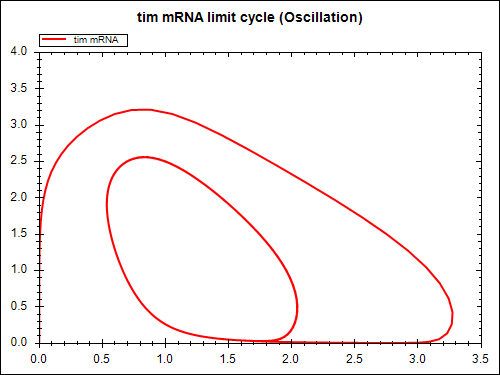
\includegraphics[width=1.0\textwidth]{examples/leloup-sbml/results/sedml_webtools/plot2}
         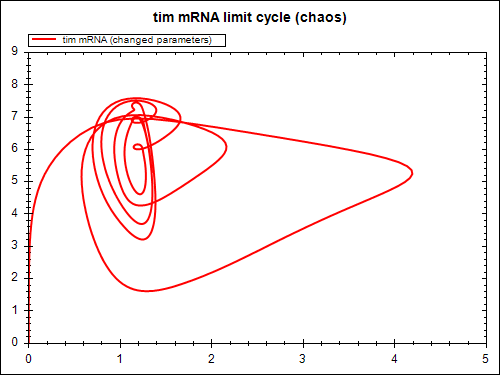
\includegraphics[width=1.0\textwidth]{examples/leloup-sbml/results/sedml_webtools/plot3}
        \caption{The simulation result gained from the simulation description given in \lst{leloup-sbml} with SED-ML webtools.}
    \end{minipage}\hfill
    \begin{minipage}{0.47\textwidth}
        \centering
        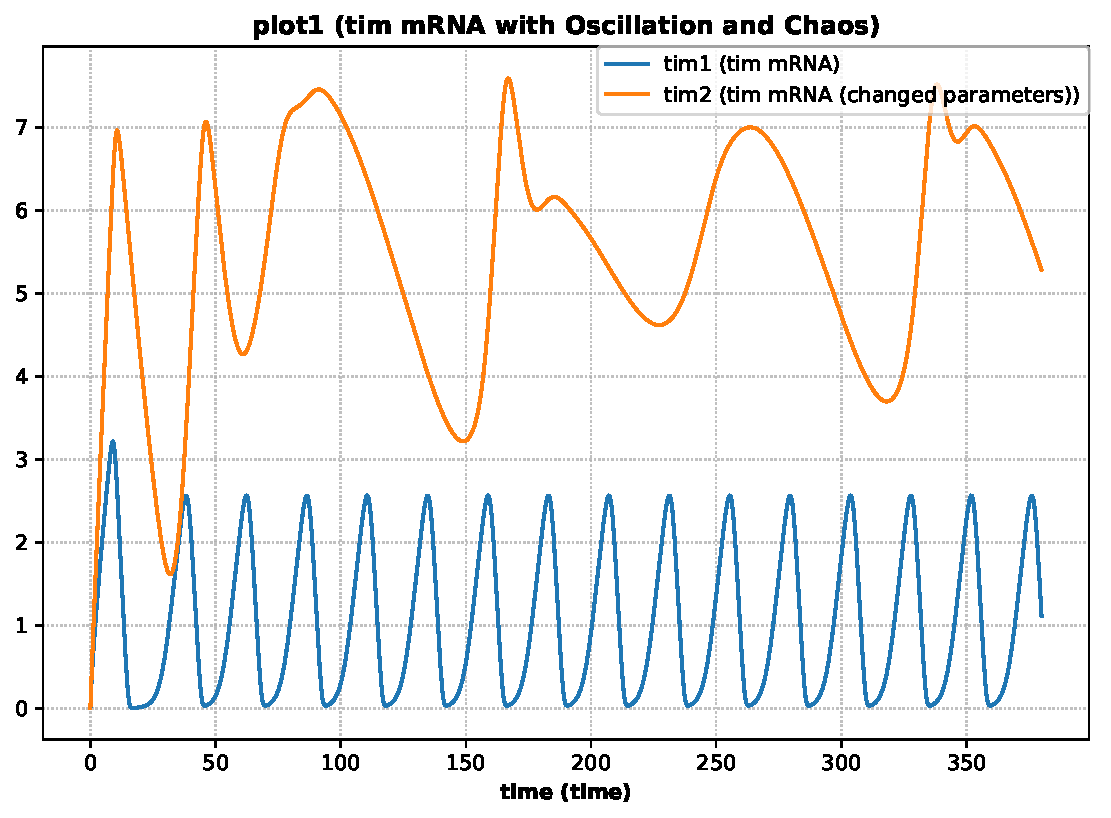
\includegraphics[width=1.0\textwidth]{examples/leloup-sbml/results/tellurium/plot1}
         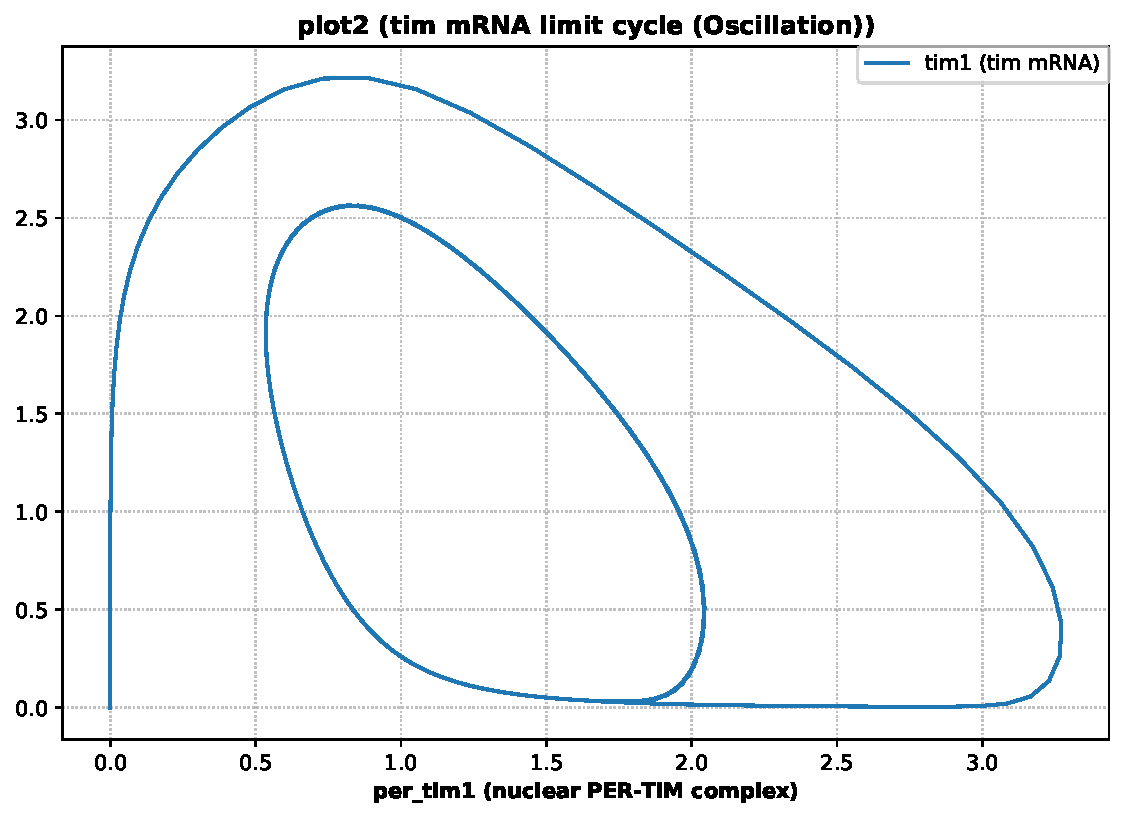
\includegraphics[width=1.0\textwidth]{examples/leloup-sbml/results/tellurium/plot2}
         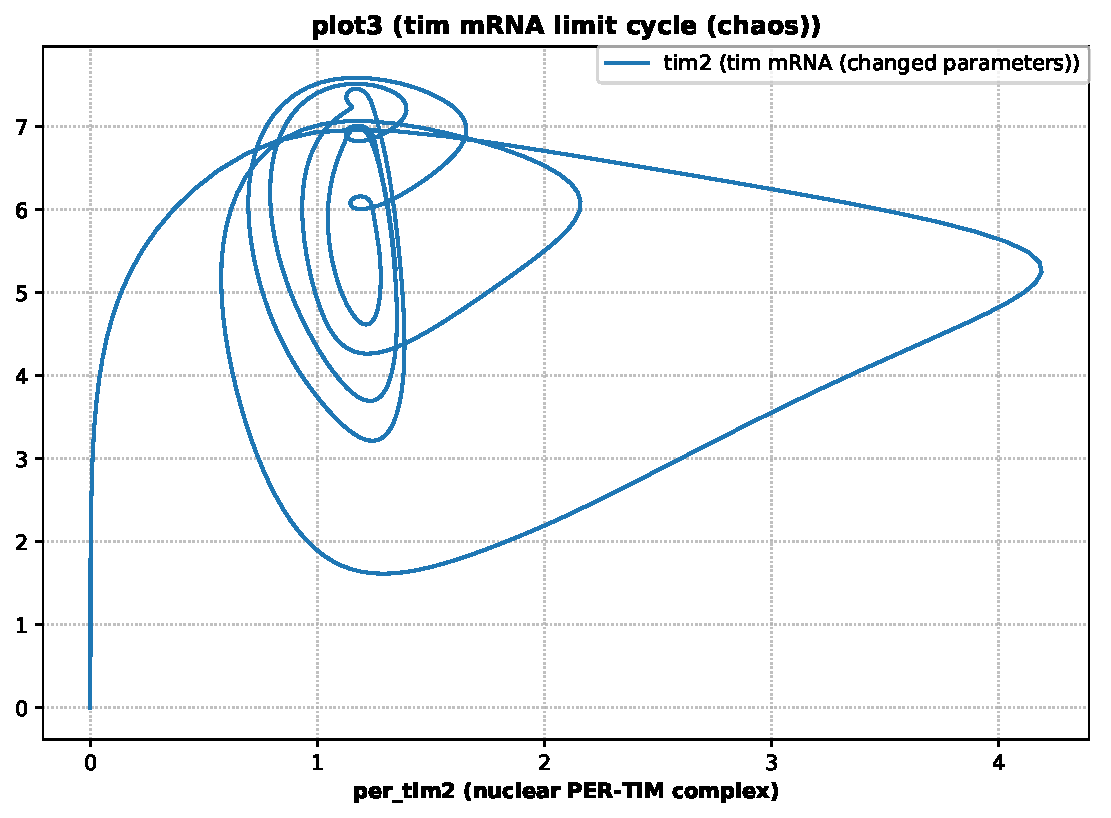
\includegraphics[width=1.0\textwidth]{examples/leloup-sbml/results/tellurium/plot3}        
        \caption{The simulation result gained from the simulation description given in \lst{leloup-sbml} with tellurium.}
    \end{minipage}
    \label{fig:leloup-sbml}
\end{figure}

\myXmlImport{LeLoup Model Simulation Description in SED-ML}{lst:leloup-sbml}{examples/leloup-sbml/leloup-sbml.xml}


% ~~~ LE LOUP (CELLML) ~~~
\subsection{Le Loup Model CellML (\code{leloup-cellml.omex})}
\label{example:leloup_cellml}

\hl{TODO: add better cellml example which can be executed with existing software, i.e. OpenCOR. The current example is not working or runnable. This must be replaced.}

The following example provides a SED-ML description for the simulation of the model based on the publication \citep{LeLoup1999}. Whereas the \hyperref[example:leloup_sbml]{previous example} used SBML to encode the simulation experiment, here the model is taken from the CellML Model Repository \citep{LLH+08}.


\sedfigX[scale=0.6]{examples/leloup-cellml/results/leloup-cellml}{The simulation result gained from the simulation description given in \lst{leloup-cellml}}{fig:leloup-cellml}

\myXmlImport{LeLoup Model Simulation Description in SED-ML}{lst:leloup-cellml}{examples/leloup-cellml/leloup-cellml.xml}
